\documentclass[a4paper]{article}
\usepackage[utf8]{inputenc}
\usepackage[italian]{babel}
\usepackage[T1]{fontenc}
\usepackage{amsmath,amssymb,amsthm}
\usepackage{enumerate}
\usepackage{epigraph}
\usepackage{fontspec}
\usepackage{graphicx}
\usepackage{hyperref}

\graphicspath{ {./images/} }

\title{
  {
    \fontspec[ Path = fonts/ ]{Symbola}
    \symbol{"1F17C}\symbol{"1F435}\symbol{"1F17D}\symbol{"1F17A}ey
  } \large \\
  \small Relazione del progetto per l'insegnamento di Algoritmi e strutture di
  dati
}

\author{
  Gaia Clerici (\#971338),
  Stefano Volpe (\#969766)
}

\date{
	Universit\`a di Bologna \\
  \today
}

\begin{document}

\maketitle

\begin{figure}[h]
  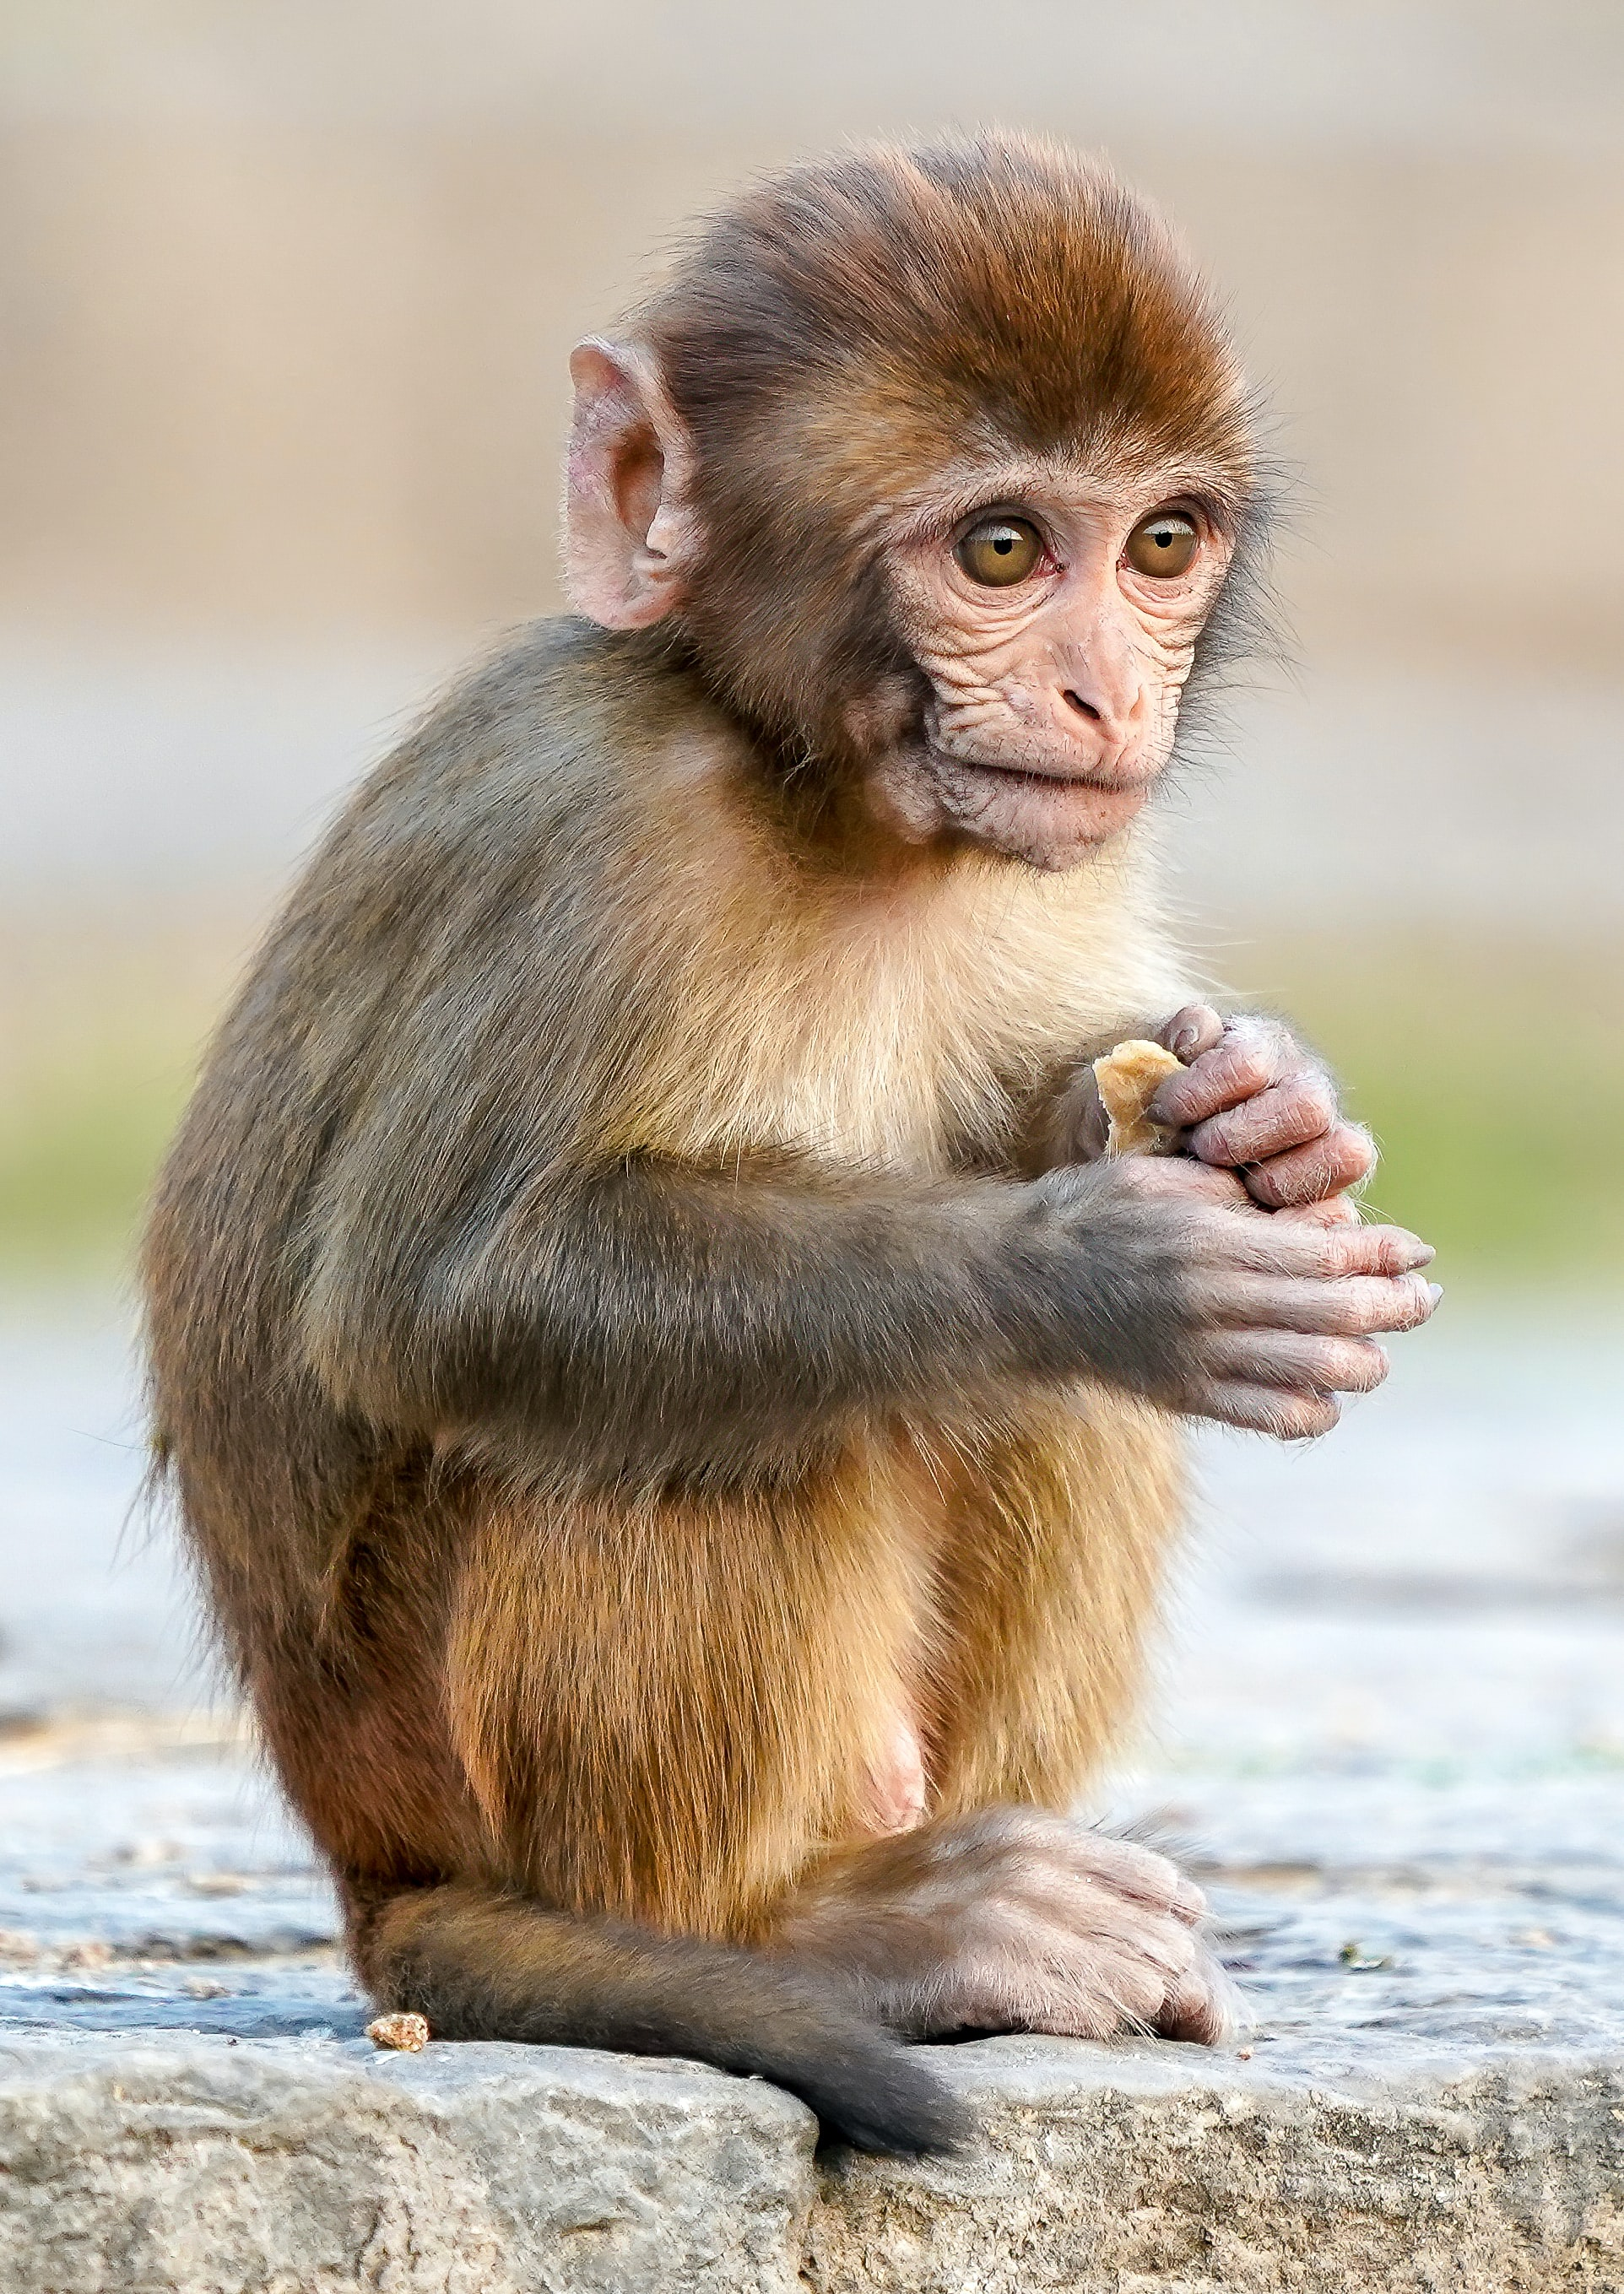
\includegraphics[width=0.75\textwidth]{monkey}
  \centering
  \caption{\href{https://unsplash.com/photos/daC7ji1EMHM}{una scimmia
  (foto di Bob Brewer)}}
\end{figure}

\pagebreak

\epigraph{Fa' la brava scimmietta.}{\textit{L'uomo con il cappello giallo}}

\tableofcontents

\section{Specifiche}

\subsection{Il gioco: \emph{m,n,k-game}}

Il gioco \emph{m,n,k-game} è deterministico, a turni, a due giocatori, a somma
zero e con informazione perfetta. In una partita, i due agenti si alternano nel
marcare una cella vuota in una griglia di dimensione \emph{m} \times \emph{n}
con un simbolo del proprio colore. Se un giocatore allinea in orizzontale,
verticale o diagonale almeno \emph{k} simboli, questi vince la partita e il suo
avversario la perde. Se non rimangono più celle vuote sulla griglia, la partita
finisce in pareggio.

\subsection{Il metagioco: il torneo}

Ogni volta che, all'interno del torneo, un giocatore conclude una partita, egli
guadagna: 
\begin{itemize}
  \item 3 punti in caso di una vittoria come secondo giocatore, ma non a tavolino;
  \item 2 punti in caso di una vittoria come primo giocatore o a tavolino;
  \item 1 punto in caso di un pareggio;
  \item 0 punti in caso si una sconfitta.
\end{itemize}

\noindent 
Per ognuna delle seguenti configurazioni, ciascun giocatore del torneo gioca
esattamente quattro partite contro ogni altro partecipante, di cui due come
primo giocatore e due come secondo giocatore.

% TODO: tabella configurazioni

\subsection{Obiettivo: il giocatore}

\subsection{L'interfaccia: il pacchetto \verb!mnkgame!}

\section{Analisi del problema}

\section{Strumenti}

\section{Scelte progettuali}

\section{Conclusioni}

\section{Ricerche future}

\section{Bibliografia}

\end{document}
